% !TEX root = thesis.tex

\chapter{$\zg$+Jets at 100TeV}
\label{chap:100TeV}

	Even though the Large Hadron Collider is still in its infancy there is an ever growing effort to discuss
	where we go next as a high energy collider physics community.  A wide range of options have been put forward
	including the linear colliders Compact Linear Collider (CLIC) \cite{Abramowicz:2013tzc} and the International
	Linear Collider (ILC) \cite{BrauJames:2007aa}.  While both of these machines are designed to be precision
	electron-positron linear colliders they have very different designs; CLIC would operate at around a
	centre-of-mass energy of $3$~TeV and use cutting edge accelerating technology whereas the ILC would collide
	at $0.5$~TeV (with a possible upgrade to $1$~TeV).

	However, there are other suggestions on the table.  Of particular interest for this work is the prospect
	of a hadronic Future Circular Collider (FCC-hh).  There are other possible initial states such as
	hadron-lepton or a lepton-lepton being discussed but for obvious reasons it is the FCC-hh which we will
	focus on here.

	One particularly exciting scenario is that of a \htev hadronic collider housed in an extended tunnel
	approximately $100$~km in circumference at the CERN site in Geneva.  Such a machine would make an
	excellent `discovery machine' since it would cover a vast range in partonic centre-of-mass energies.
	The energies probed here would be orders of magnitude higher than ever seen at a hadronic collider
	and so this would be an invaluable test of high scale QCD.  Similarly to physics at the current LHC
	the dominant background would be QCD in nature and so in order for us to be able to extract useful
	information about potential new physics we would need to be able to model this QCD background with
	incredible precision.  Current state-of-the-art for many QCD processes is still limited to next-to-leading
	order in $\alpha_s$ although progress is being made towards improving this to next-to-next-to-leading
	order in some key physics processes, for example Higgs production via gluon fusion is known at N3LO \cite{Anastasiou:2015ema}.
	However, as in the preceding chapters we will instead investigate the effects of the higher-order
	logarithmically enhanced contributions to the perturbative series.  As discussed in chapter \ref{chap:theory}
	these terms are not all captured by NNLO (or any fixed-order scheme $\text{N}^m$LO for that matter).

	The results of chapters \ref{chap:Zs} and \ref{chap:ATLAS} clearly show that these effects are already important
	at a the \stev for both dijets and $\zg$+dijets respectively.  We therefore expect that at a \htev FCC-hh we would
	see a greater effect from the terms enhanced in the High Energy limit beyond a fixed-order only prediction.

	Here we present a study of $\zg$+dijets at a centre-of-mass energy of \htev.  The final state cuts
	are outlined in table~\eqref{tab:atlascuts100}.  For each figure we show the equivalent result calculated
	at \stev with a jet $p_T$ cut of $30$~GeV (which was found to be in excellent agreement with data) as
	well as the \htev predictions for jet cuts of $30$~GeV, $60$~GeV and $100$~GeV.  The choice of jet cut
	is an interesting problem since it the best variable for weeding out physics other than the hard
	perturbative scatter.  For example, even at the \stev LHC a QCD study with a jet cut of, say,
	$10$~GeV would be as much a test of our theoretical understanding of perturbative physics as it would
	a test of our descriptions for parton showers, multiple parton interactions and underlying event.
	While this is a perfectly valid analysis to do it is \emph{not} the best choice if our aim is to
	improve our understanding of perturbative QCD.  The same argument applies for a \htev collider
	only more so!  As we go to increasingly higher centre-of-mass energies we may need to raise our
	jet cuts so as to ensure the data we hope to describe is as unpolluted as possible.  Each figure
	also shows the ratio of the \htev prediction to the \stev prediction to emphasise any features
	which may otherwise be hard to see - such as changes in shape.

	\begin{table}[bth]
	  \centering
	  \begin{tabular}{|l|c|}
	    \hline
	    Lepton Cuts & $p_{T\ell}>20$~GeV, \; $|\eta_\ell|<2.5$ \\
	    & $\Delta R^{\ell^+\ell^-} > 0.2$, \; $66$~GeV $\leq m^{\ell^+\ell^-} \leq
	      116$~GeV \\ \hline
	    $7$~TeV Jet Cuts (anti-$k_T$, 0.4) & $p_{Tj}>$ {\color{Purple}$30$~GeV} \\
	    &  $|y_j|<4.4$, \;$\Delta R^{j\ell} >0.5$,  \\ \hline
	    $100$~TeV Jet Cuts (anti-$k_T$, 0.4) & $p_{Tj}>$ {\color{Red}$30$~GeV}, {\color{ForestGreen}$60$~GeV}, {\color{blue}$100$~GeV} \\
	    &  $|y_j|<4.4$, \;$\Delta R^{j\ell} >0.5$,  \\ \hline
	  \end{tabular}
	  \caption{Cuts applied to theory simulations for the \htev
	    $Z$-plus-jets analysis results shown in Figs.~\eqref{fig:100tev_12a}--\eqref{fig:100tev_10b}.  We apply only one
	    jet cut of 30~GeV to the jets in the 7~TeV analysis but separately study the 100~TeV jets with cuts of
	    30~GeV, 60~GeV and 100~GeV shown in red, green and blue respectively.}
	  \label{tab:atlascuts100}
	\end{table}

	We begin by discussing what is by far the most uninteresting figure in this thesis (at least at first glance!).
	Fig.~\eqref{fig:100tev_12a} shows the differential distribution in the azimuthal separation of the
	two leading jets in $p_T$, $\Delta\phi_{j1, j2}$.  It is clear that although the cross-section of the \htev
	study with 100~GeV jets is significantly greater than that of the \stev result the increase in cross-section is uniform
	throughout the range of $\Delta\phi_{j1, j2}$ - this is clear from the ratio.  What makes the uninteresting
	fig.~\eqref{fig:100tev_12a} so interesting is that if QCD behaved exactly the same at \htev as it did at \stev
	we would expect all of the plots in this chapter to have a ratio line which was a perfectly straight line
	which merely reflected the increase in cross-section.  However, this turns out not to be the case.  We can also see
	that as we increase the minimum $p_\perp$ requirements in the \htev study we the cross-section decrease, as of course
	we expect it to do, and we induce a more interesting behaviour in the ratio of the predictions to the \stev line.
	This can be easily understood since as we force the jets to higher values of transverse momenta the back-to-back
	topology becomes more favourable and hence more of the total cross-section is found at $|\Delta\phi^{j1, j2}|\approx\pi$.

	\begin{figure}[bth]
		\centering
		\begin{subfigure}[b]{0.49\textwidth}
			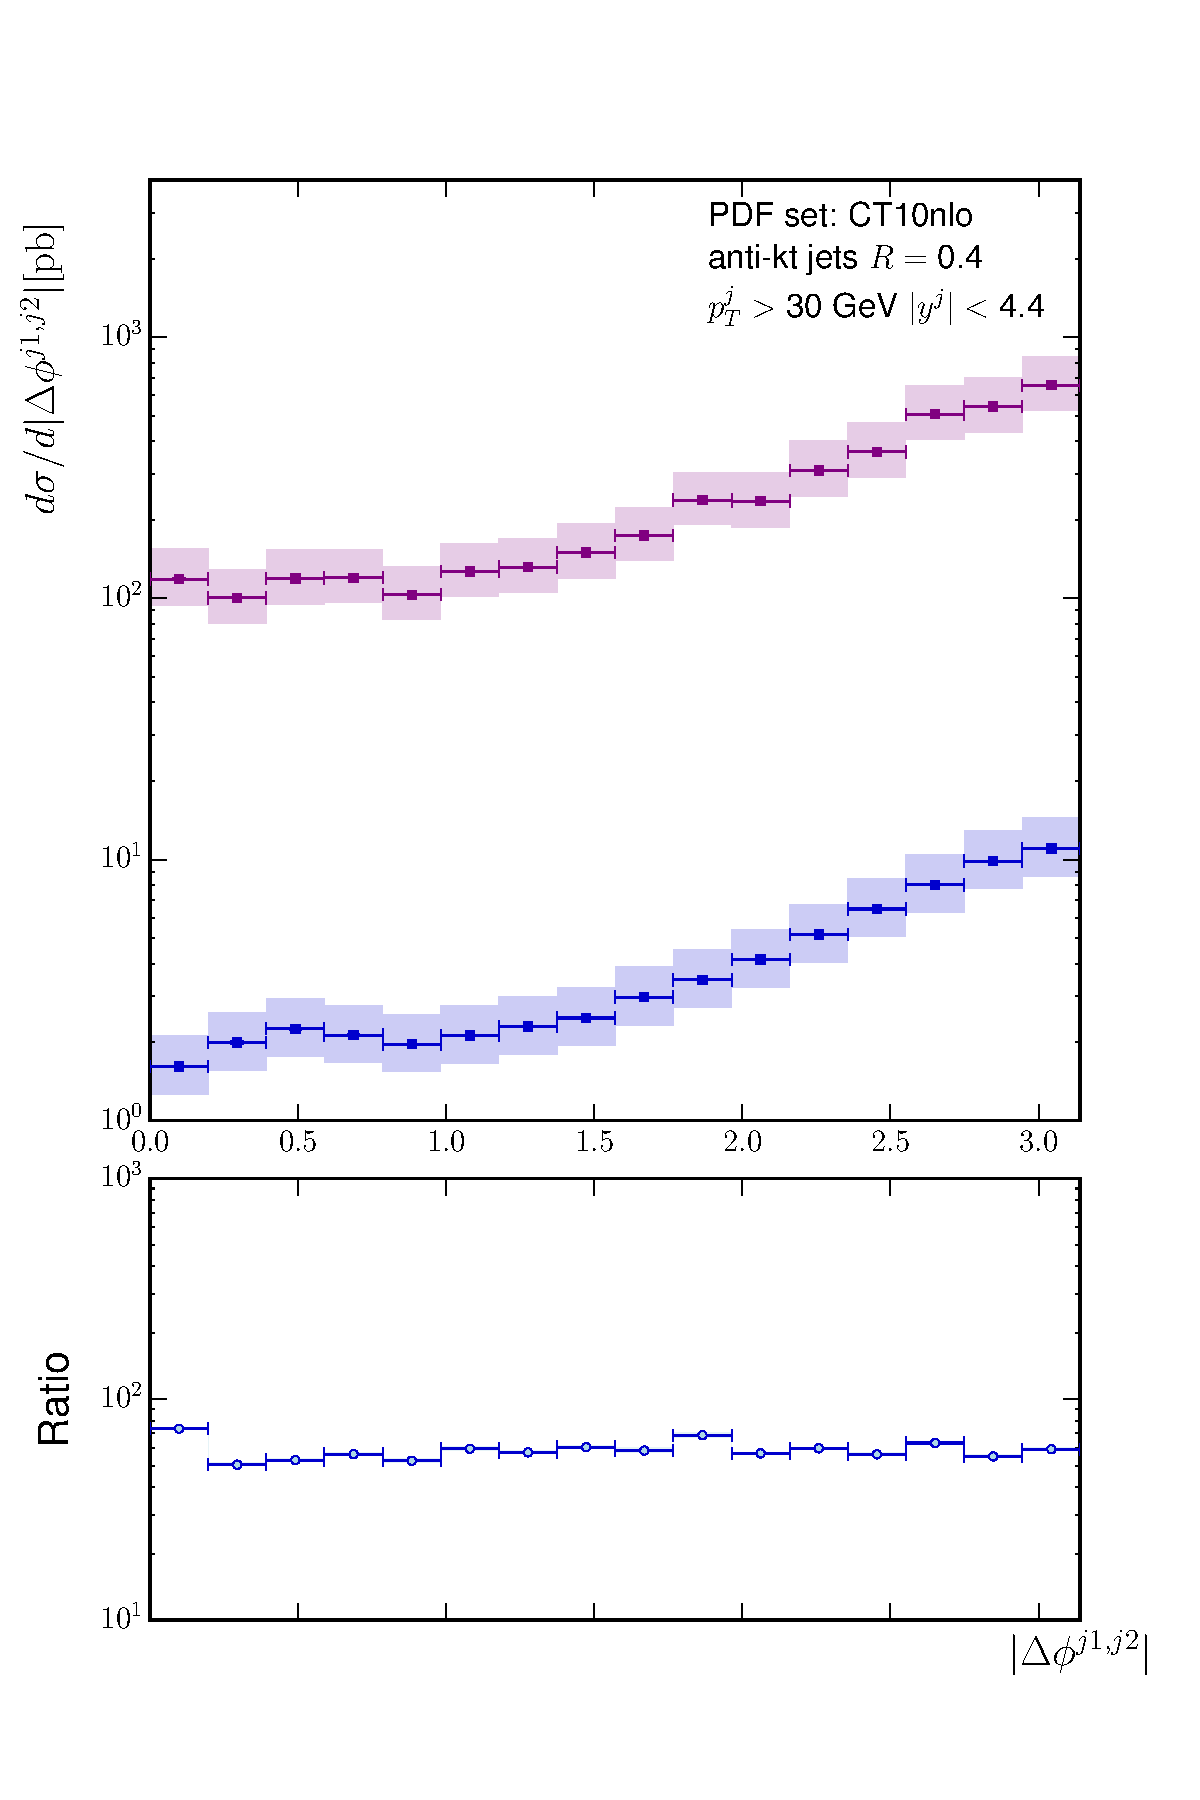
\includegraphics[width=\textwidth]{ATLAS_Z_100TeV_12a}
			\caption{}
			\label{fig:100tev_12a}
		\end{subfigure}
		\begin{subfigure}[b]{0.49\textwidth}
			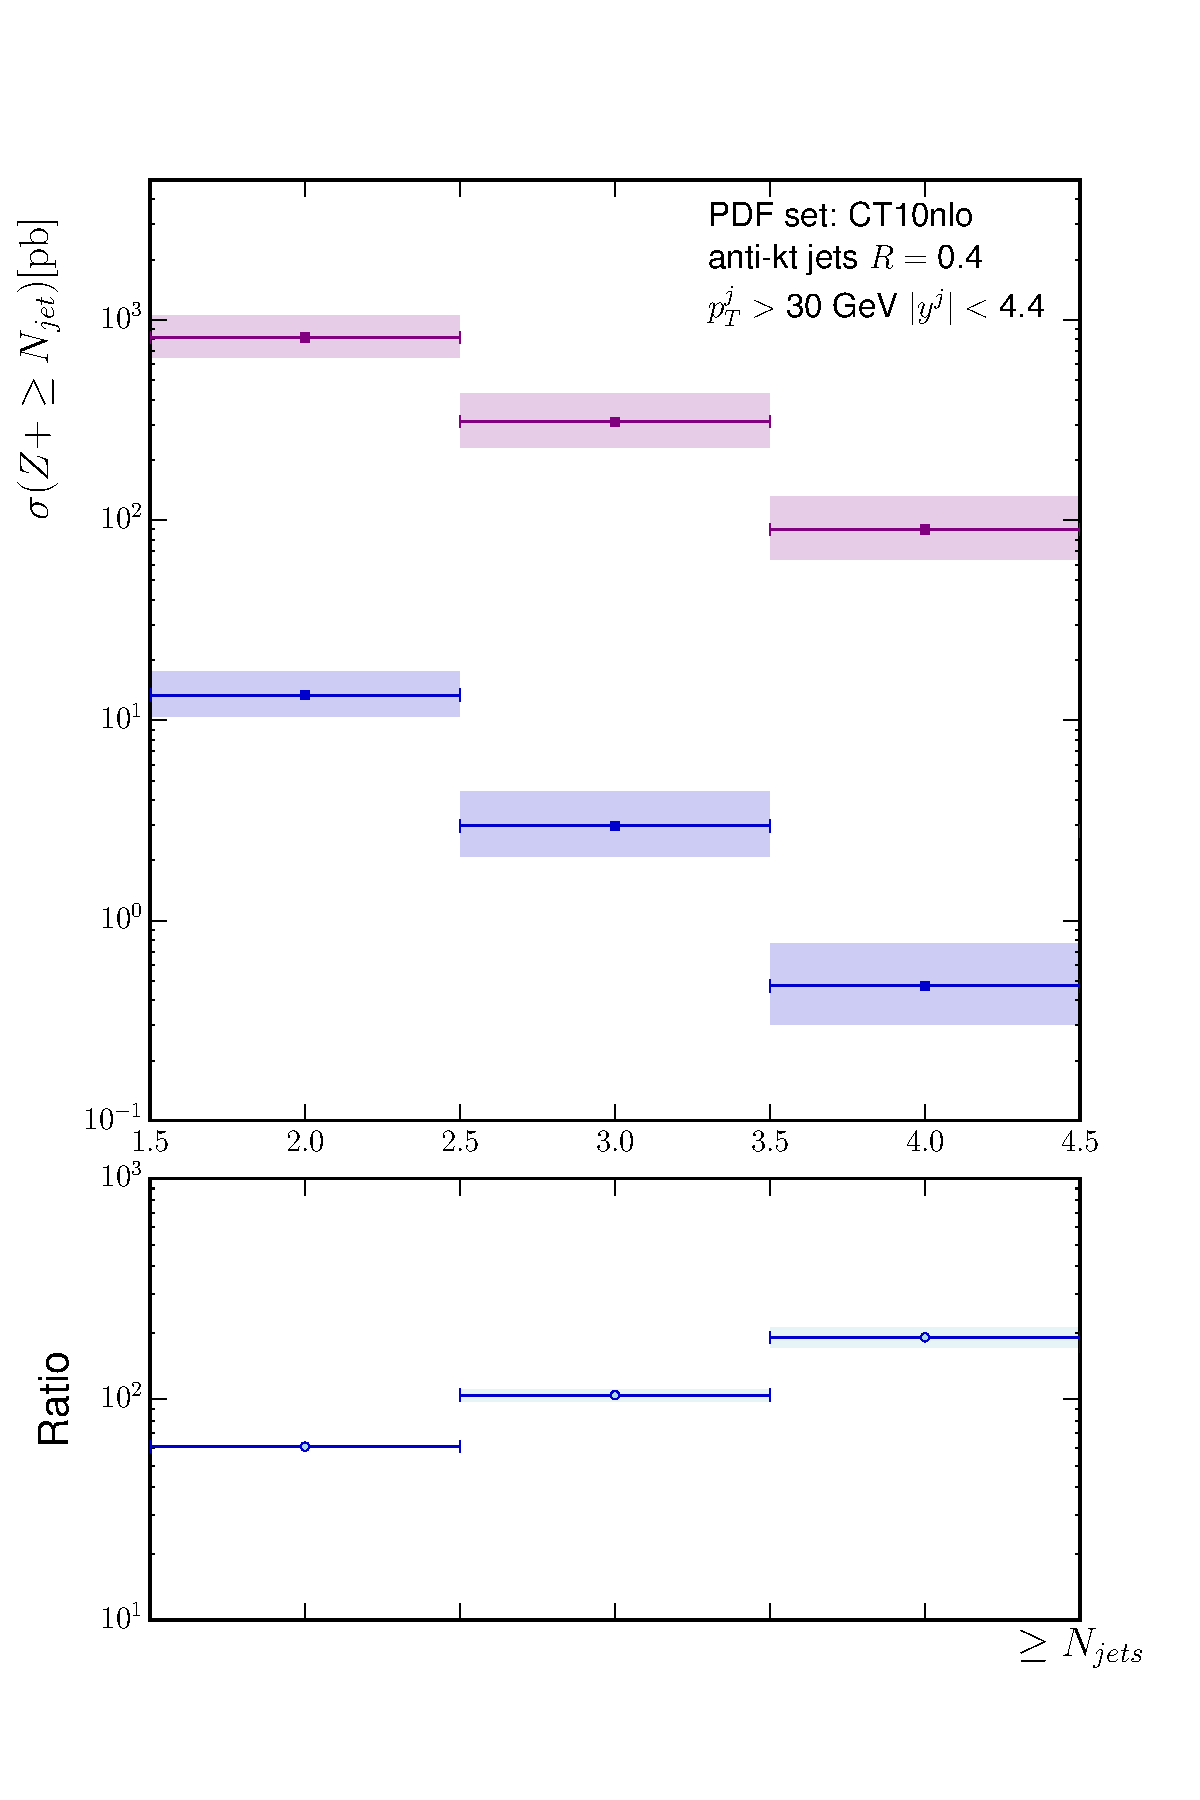
\includegraphics[width=\textwidth]{ATLAS_Z_100TeV_2a}
			\caption{}
			\label{fig:100tev_2a}
		\end{subfigure}
		\caption{Fig.~\eqref{fig:100tev_12a} - The differential cross-section for $\zg$ plus inclusive dijets as a
		function of the azimuthal separation of the dijet system shown for centre-of-mass energies of 7TeV (blue)
		and 100TeV (pink). Fig.~\eqref{fig:100tev_2a} - The cross-section for $\zg$ plus inclusive dijets as a
		function of the number of jets, $N_{\text{jet}}$, shown for centre-of-mass energies of 7TeV (blue) and
		100TeV (pink).}
	\end{figure}

	Fig~\eqref{fig:100tev_2a} shows the breakdown of the $\zg$+dijets cross-section in terms of the inclusive number
	of jets, $N_{\text{jet}}$.  Once again we see that the total integrated cross-section grows as we
	go to higher energy but we also see, at least for the 30~GeV jets, that the relative contribution to the cross-section
	increases as we go to higher jet multiplicity.  This is direct evidence that the convergence of the
	QCD perturbative expansion worsens as we go to higher energy.  Clearly then resummation effects
	such as those described by \hej become more important at a prospective FCC-hh machine and will need
	to be included not only in order to understand the QCD background well enough to extract and
	study new physics but also in order for precision tests of QCD.  As we increase the jet cut to 60~GeV
	we see that the ratio with respect to the \stev prediction becomes a little flatter and at a cut of 100~GeV
	the prediction is identical to that at \stev save for an extra order of magnitude in the total cross-section.
	We can understand this by considering the effect of requiring high transverse momenta on rapidity and therefore
	rapidity gaps; it is energetically very expensive to emit high $p_\perp$ radiation outside of the $y_j\approx0$ region
	and therefore we can suppress the effects of the logarithmic corrections by limiting the access to phase-space
	where they are most important.

	Fig~\eqref{fig:100tev_11a} shows the differential distribution in the absolute value of the
	rapidity span between the two leading jets in $p_T$, $\Delta y^{j1, j2}$.  We see that as we go to
	large rapidity gaps between the dijets the relative increase in the cross-section grows by almost a
	factor or $10$ as we pull the hardest two jets apart in rapidity.  This is precisely the effect of
	the logarithmic corrections since, as we saw in chapter~\ref{chap:HEQCD}, we have that:

	\begin{equation}
		\Delta y^{j1, j2}\sim \ln\left(\frac{s}{-t}\right).
	\end{equation}

	Therefore to correctly describe QCD radiation patterns with large rapidity separations at an FCC
	we must capture at least these leading logarithms.  As discussed above we see that requiring harder
	jets puts limitation on the rapidity ranges available to radiation and therefore suppresses these
	effects - however, even when we only consider extremely hard jets above 100~GeV the enhancement is
	still visible and still leads to a two-fold increase in cross-section in dijet events with a large
	rapidity span.

	\begin{figure}[bth]
		\centering
		\begin{subfigure}[b]{0.49\textwidth}
			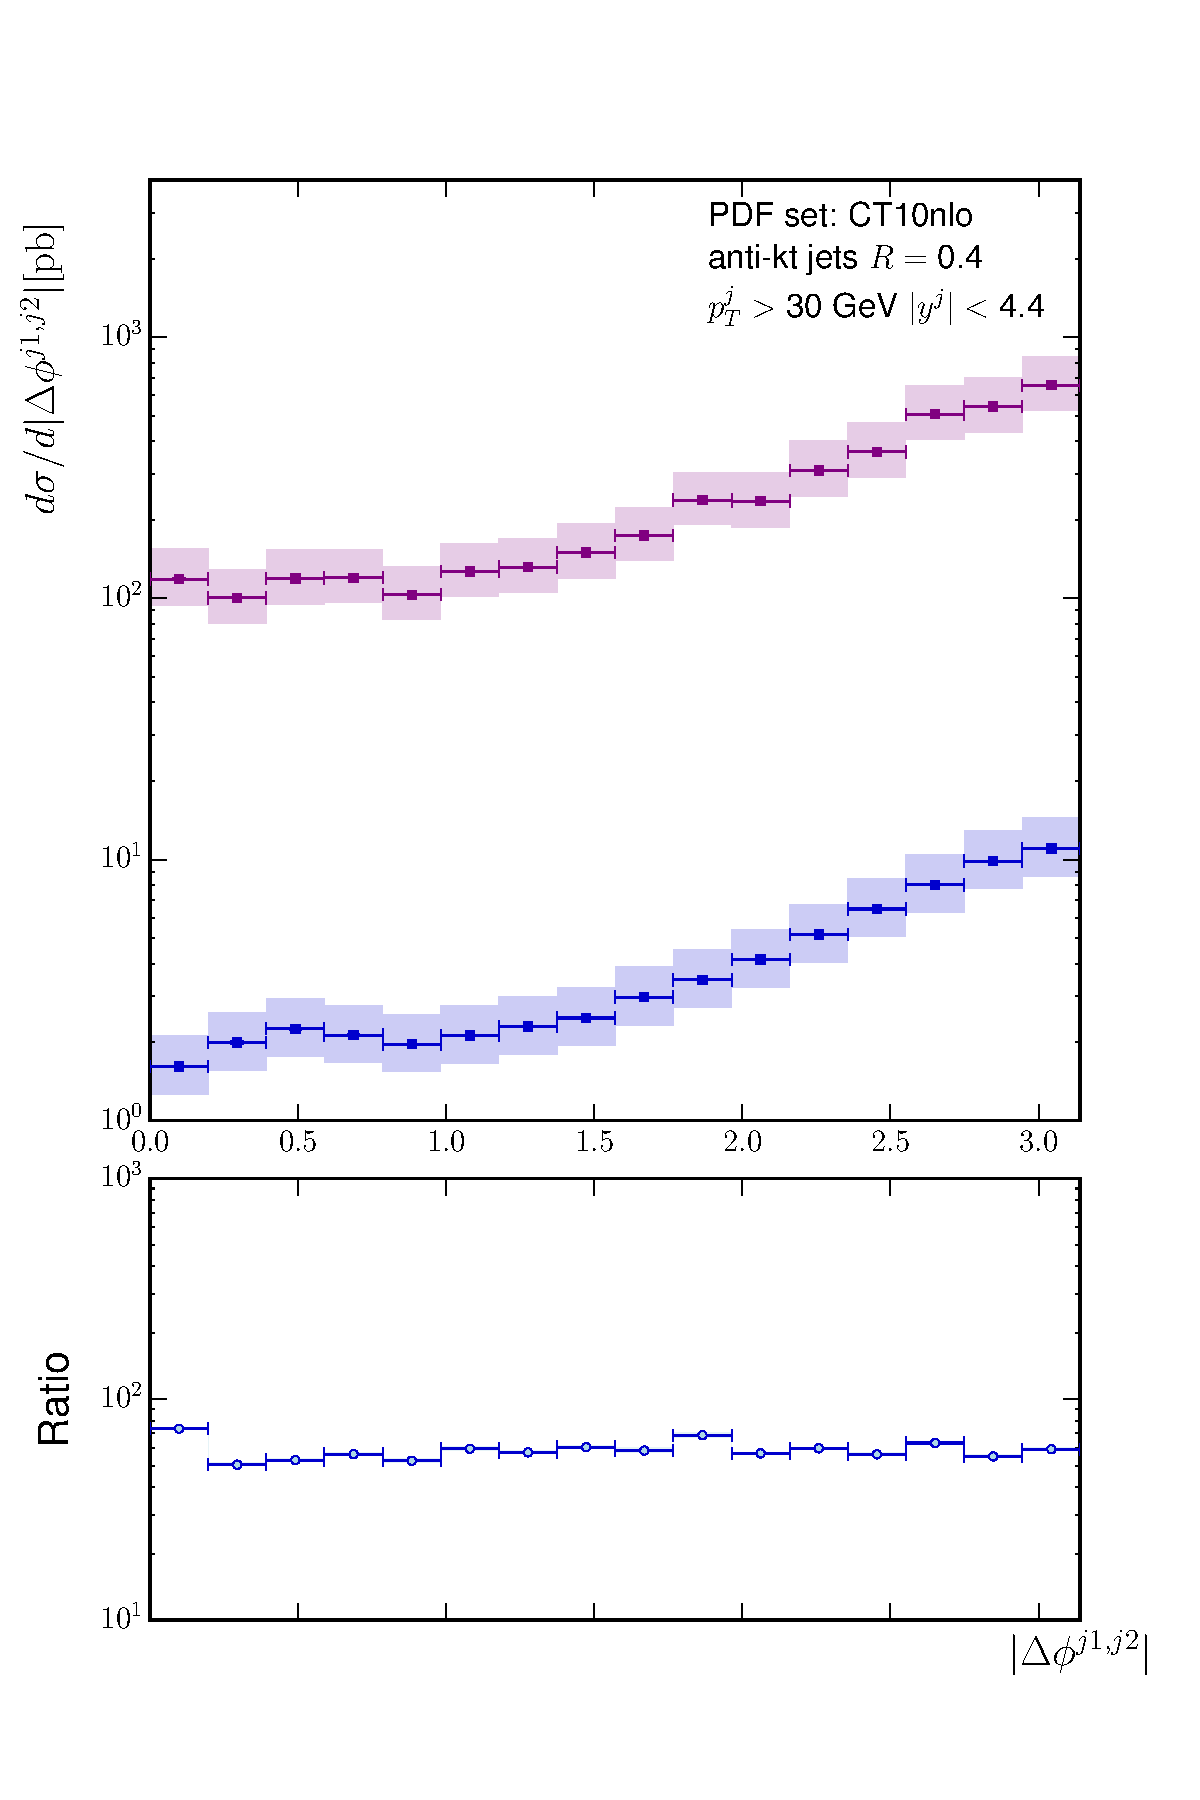
\includegraphics[width=\textwidth]{ATLAS_Z_100TeV_12a}
			\caption{}
			\label{fig:100tev_11a}
		\end{subfigure}
		\begin{subfigure}[b]{0.49\textwidth}
			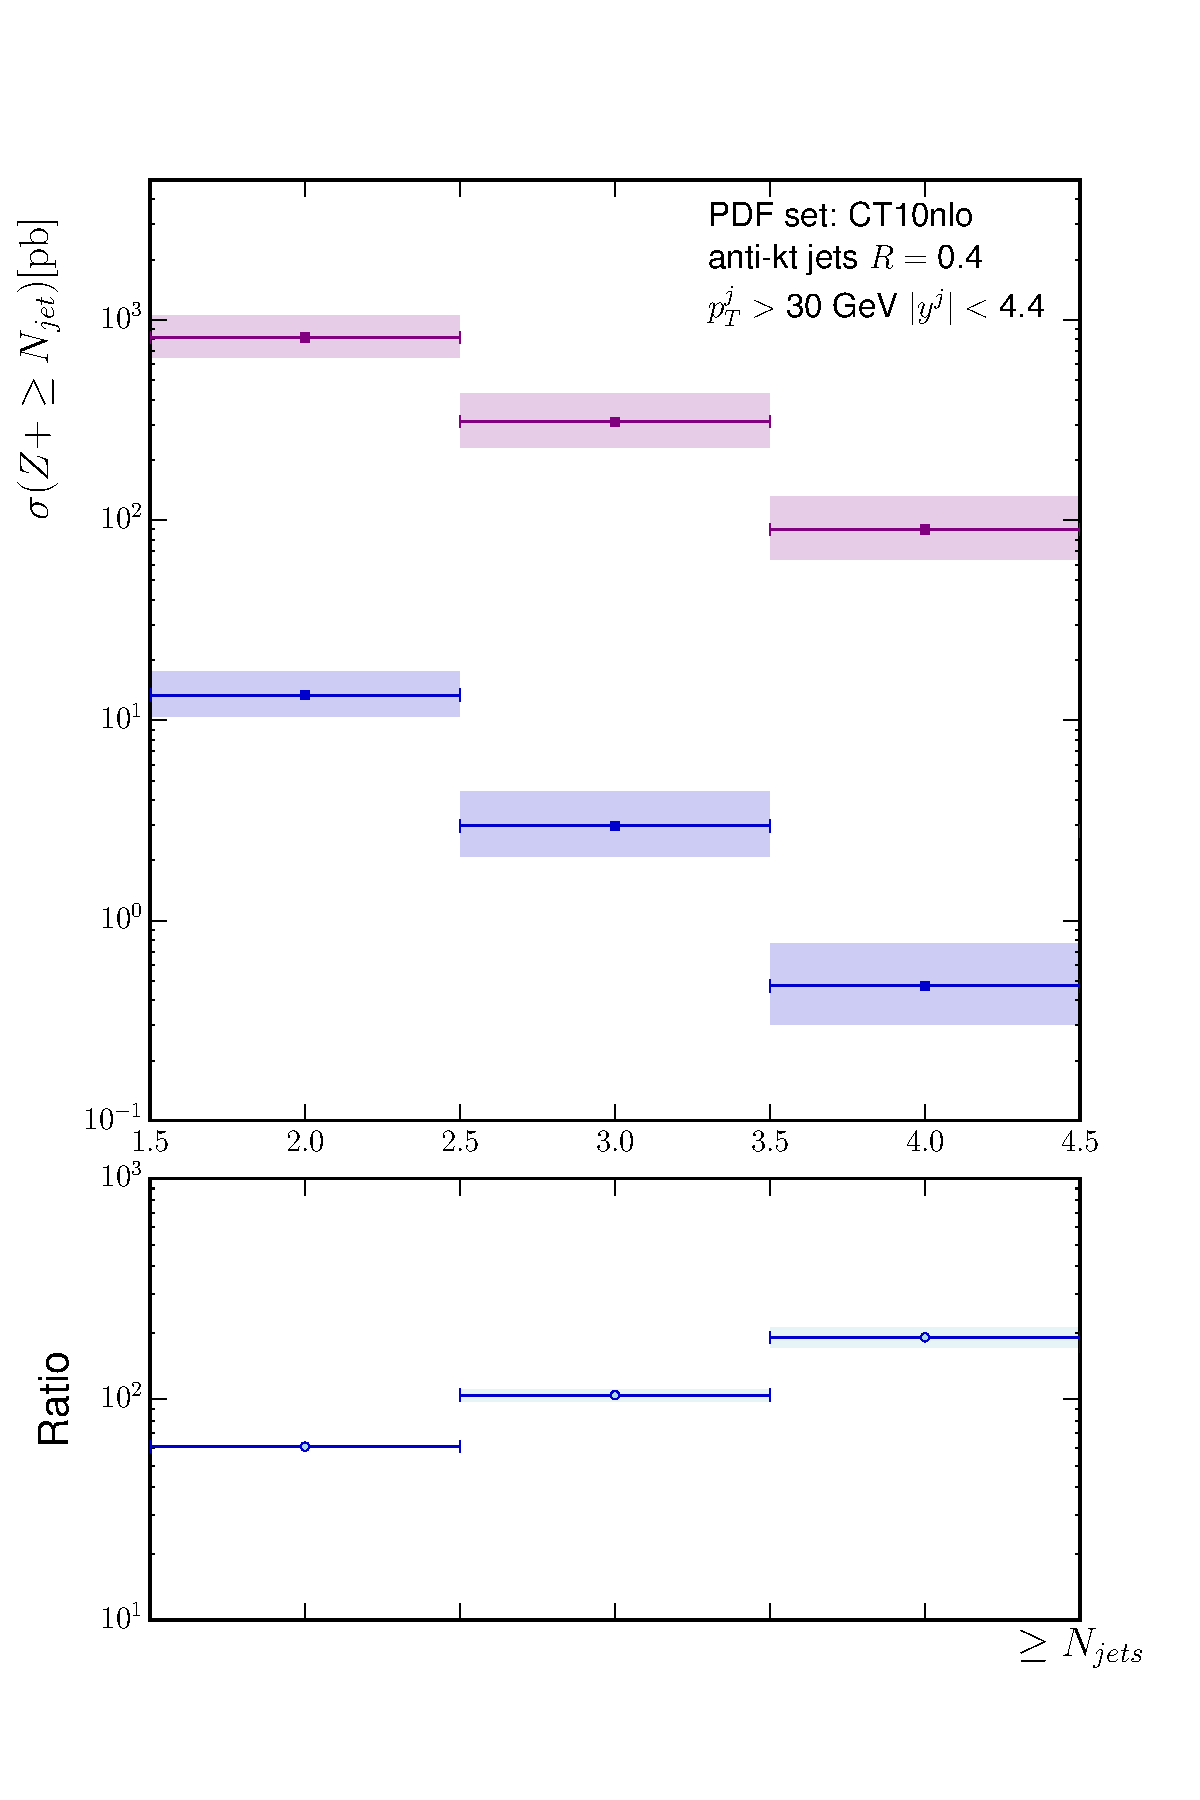
\includegraphics[width=\textwidth]{ATLAS_Z_100TeV_2a}
			\caption{}
			\label{fig:100tev_11b}
		\end{subfigure}
		\caption{Fig.~\eqref{fig:100tev_11a} - The differential cross-section for $\zg$ plus inclusive dijets as a function
		of the absolute value of the rapidity gap between the dijets, $\Delta y^{j1, j2}$ shown for centre-of-mass energies
		of 7TeV (blue) and 100TeV (pink).. Fig.~\eqref{fig:100tev_11b} - The differential cross-section for $\zg$ plus
		inclusive dijets as a function of the invariant mass of the dijets, $m^{jj}$, shown for centre-of-mass energies
		of 7TeV (blue) and 100TeV (pink).}
	\end{figure}

	In fig.~\eqref{fig:100tev_11b} we show the differential cross-section in the invariant mass of the two leading
	jets in $p_T$.  Similarly to the discussion of fig.~\eqref{fig:100tev_11a} regions of large dijet invariant mass,
	$m^{jj}$, are exactly the regions we expect to have significant higher-order perturbative corrections at play.
	Indeed, at large invariant mass there is a factor $\mathcal{O}(10)$ increase compared to systems with small
	reconstructed mass when compared to the \stev prediction.  As we make the $p_\perp$ jet cut more stringent
	we induce a large suppression at values of $m^{jj}$ equal to or below the transverse momentum cut but, more
	importantly, we see the same behaviour at very large dijet mass as for the softer cut of 30~GeV.

	\begin{figure}[bth]
		\centering
		\begin{subfigure}[b]{0.48\textwidth}
			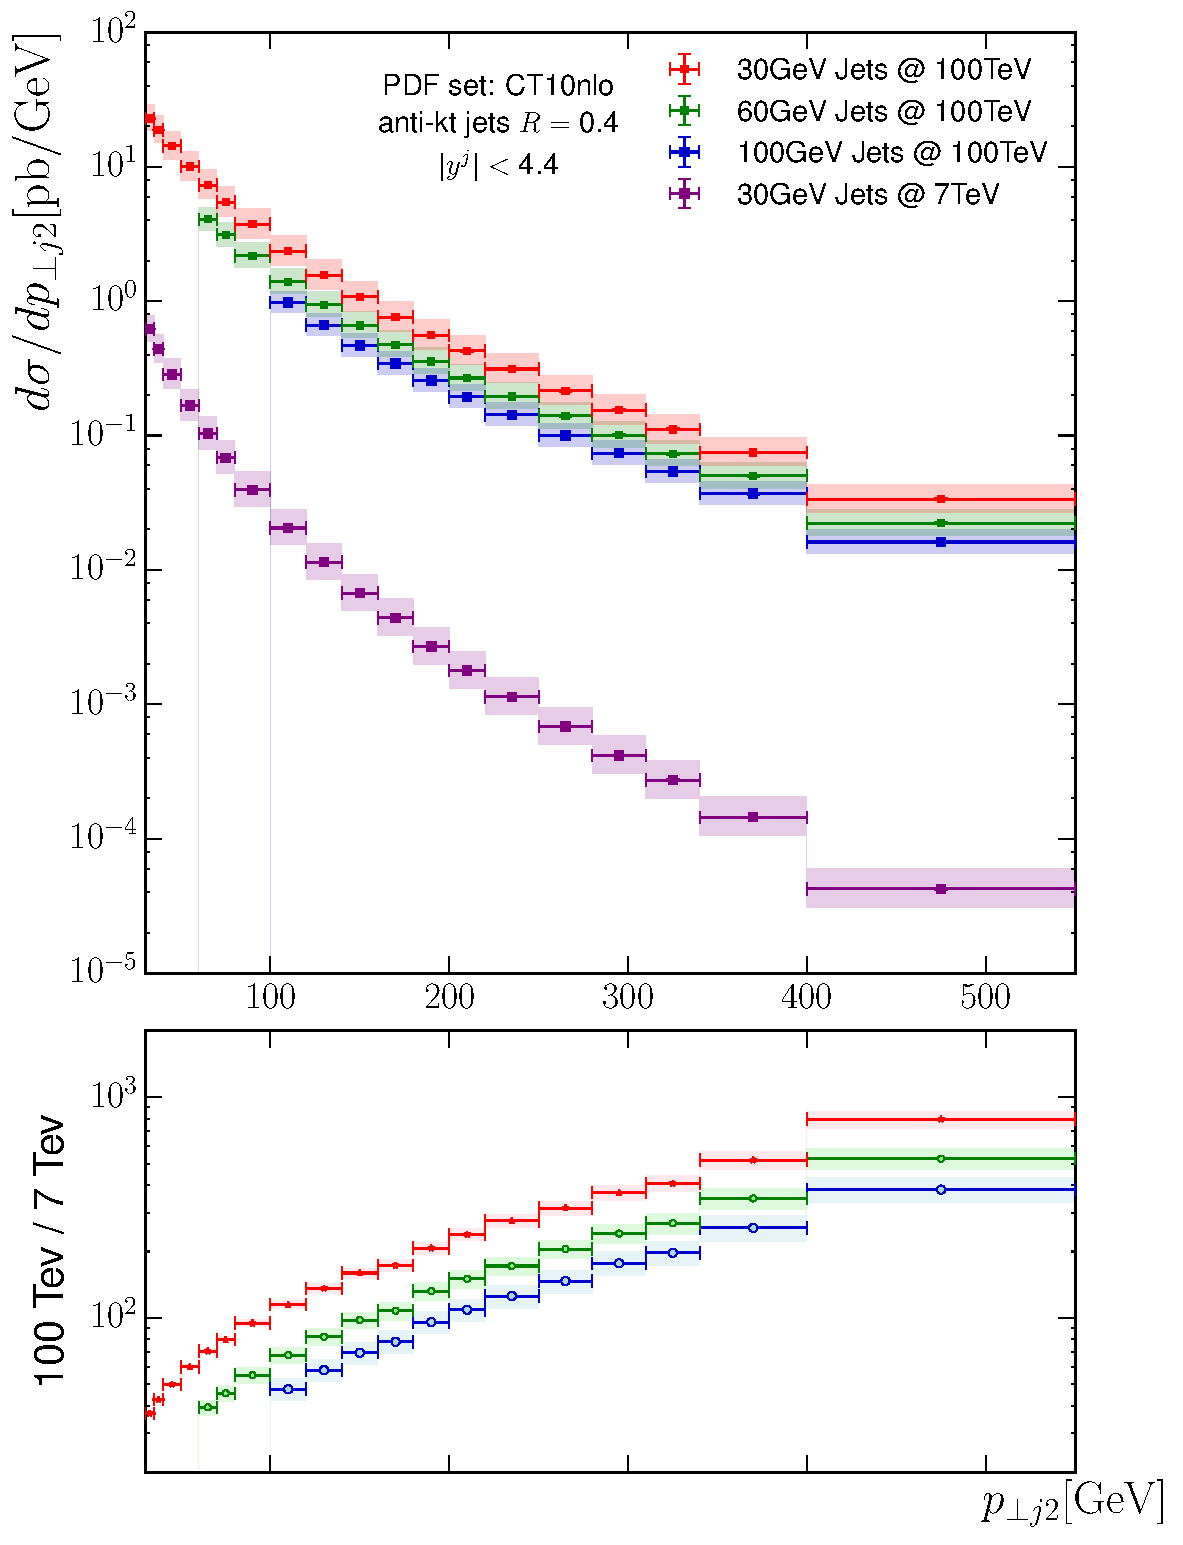
\includegraphics[width=\textwidth]{ATLAS_Z_100TeV_5b}
			\caption{}
			\label{fig:100tev_5b}
		\end{subfigure}

		\begin{subfigure}[b]{0.48\textwidth}
			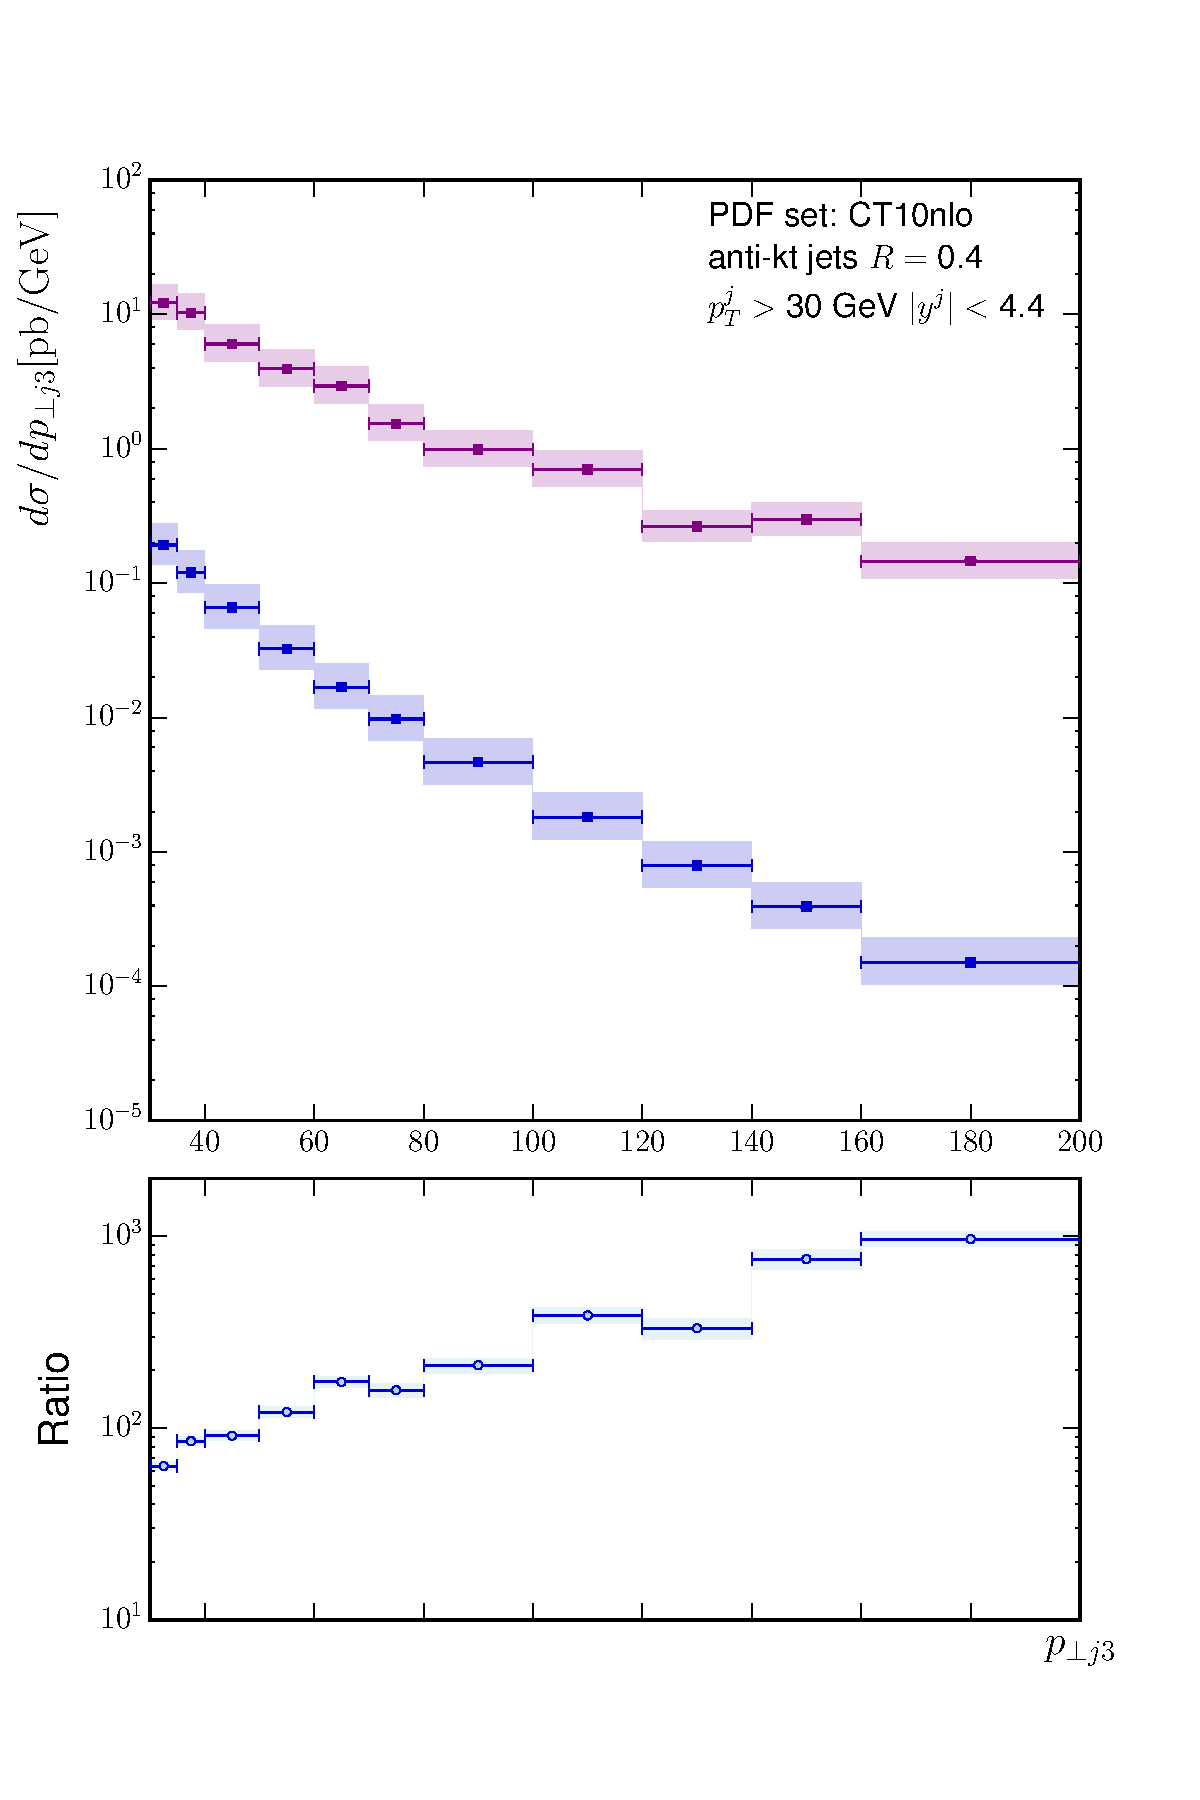
\includegraphics[width=\textwidth]{ATLAS_Z_100TeV_6a}
			\caption{}
			\label{fig:100tev_6a}
		\end{subfigure}
		~
		\begin{subfigure}[b]{0.48\textwidth}
			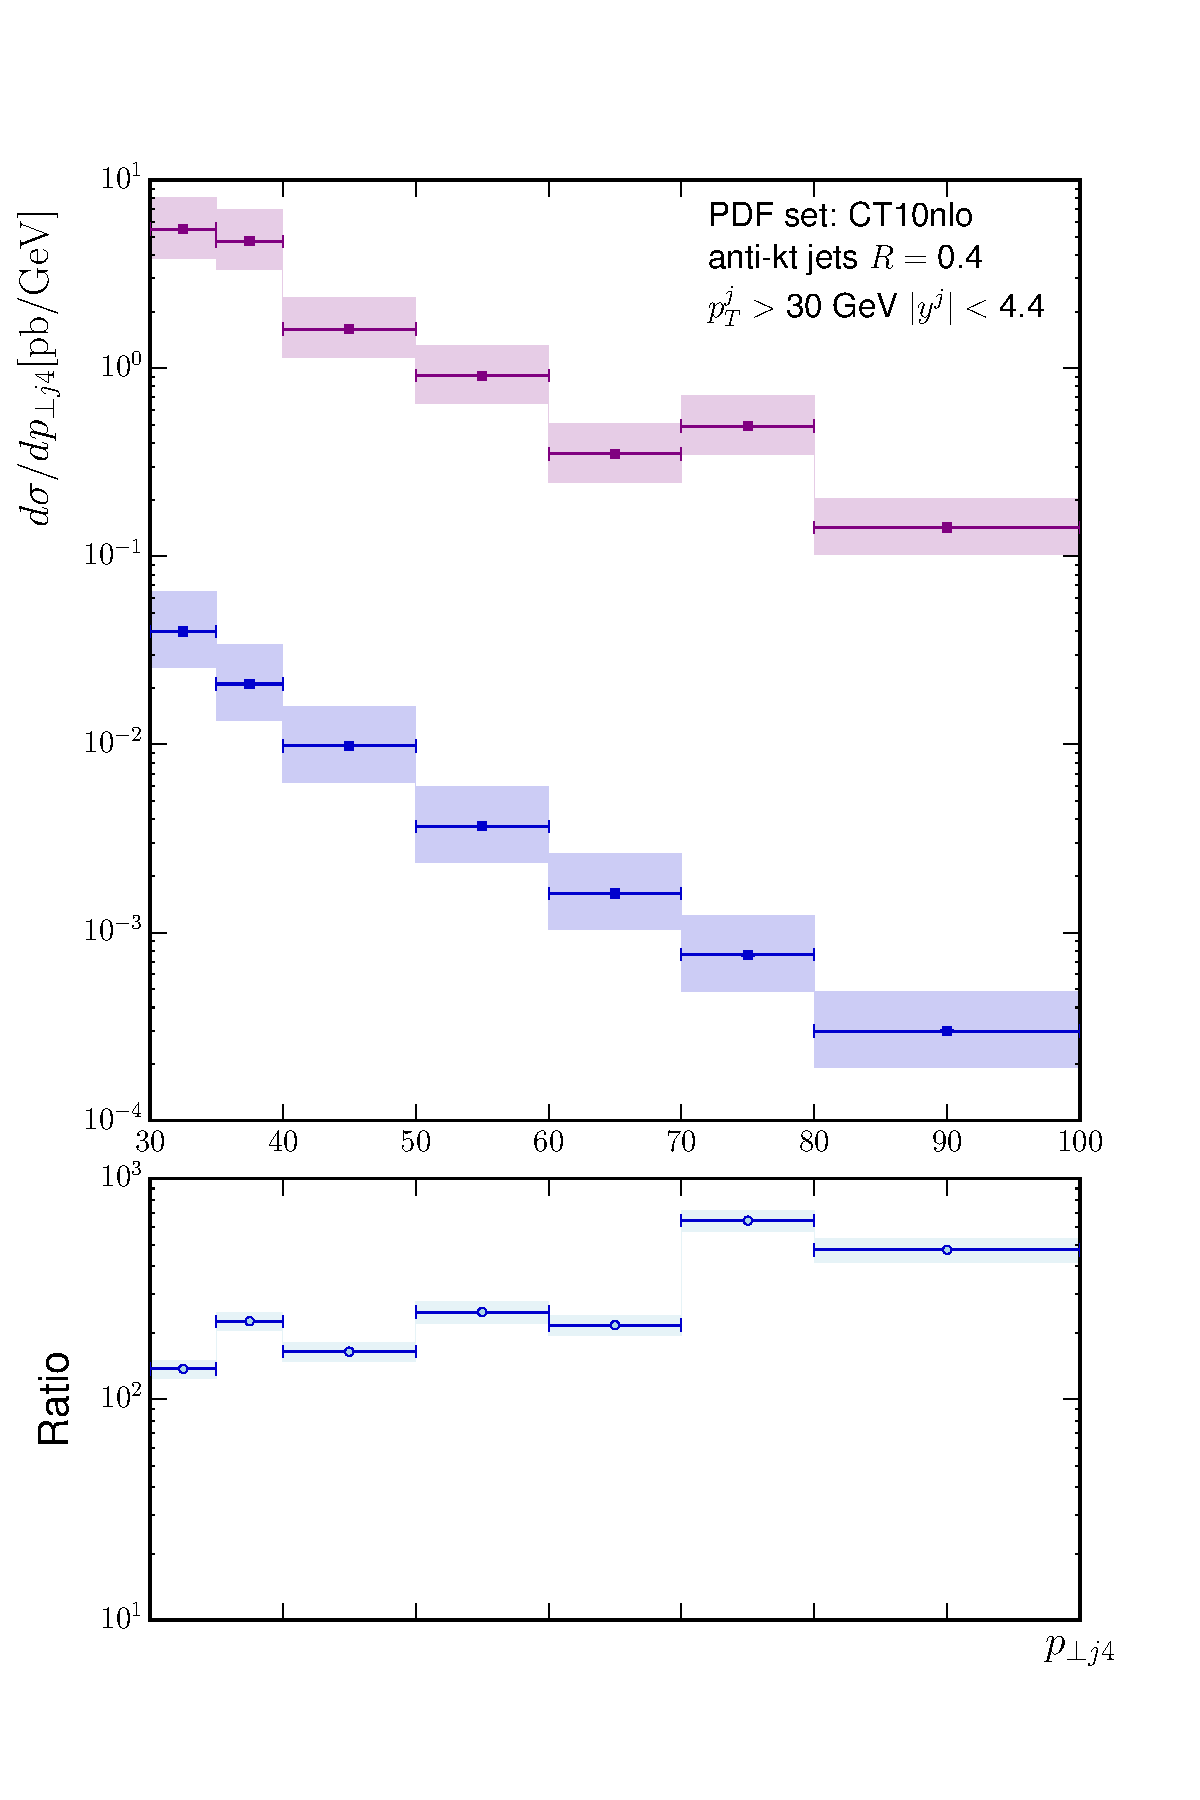
\includegraphics[width=\textwidth]{ATLAS_Z_100TeV_6b}
			\caption{}
			\label{fig:100tev_6b}
		\end{subfigure}
		\caption{The differential cross-section for $\zg$ plus inclusive dijets as a function of the transverse momentum
		         of the first, second and third leading jets in $p_T$ shown in fig. \eqref{fig:100tev_5b}, \eqref{fig:100tev_6a}
		         and \eqref{fig:100tev_6b} respectively and for centre-of-mass energies of 7TeV (blue) and 100TeV (pink).}
	\end{figure}

	Figs. \eqref{fig:100tev_5b}, \eqref{fig:100tev_6a} and \eqref{fig:100tev_6b} show the transverse momentum
	distributions for the second, third and fourth leading jet in $p_\perp$ respectively.  We observe that for all three
	variables there is a significant increase in the high $p_\perp$ region at \htev though here this can be understood
	not just in terms of an enhancement caused by logarithmic corrections but also simply because at a prospective FCC
	there would be extra energy available to radiate jets with large transverse momentum.  We see that as we move to
	60 and even 100~GeV cuts there is a small effect in the cross-section but that the shape of the ratios with respect
	to the \stev remains approximately unchanged.  Note that the 100~GeV prediction is not present in
	fig.~\eqref{fig:100tev_6b} since all the events have been cut from the studied region.

	\begin{figure}[bth]
		\centering
		\begin{subfigure}[b]{0.48\textwidth}
			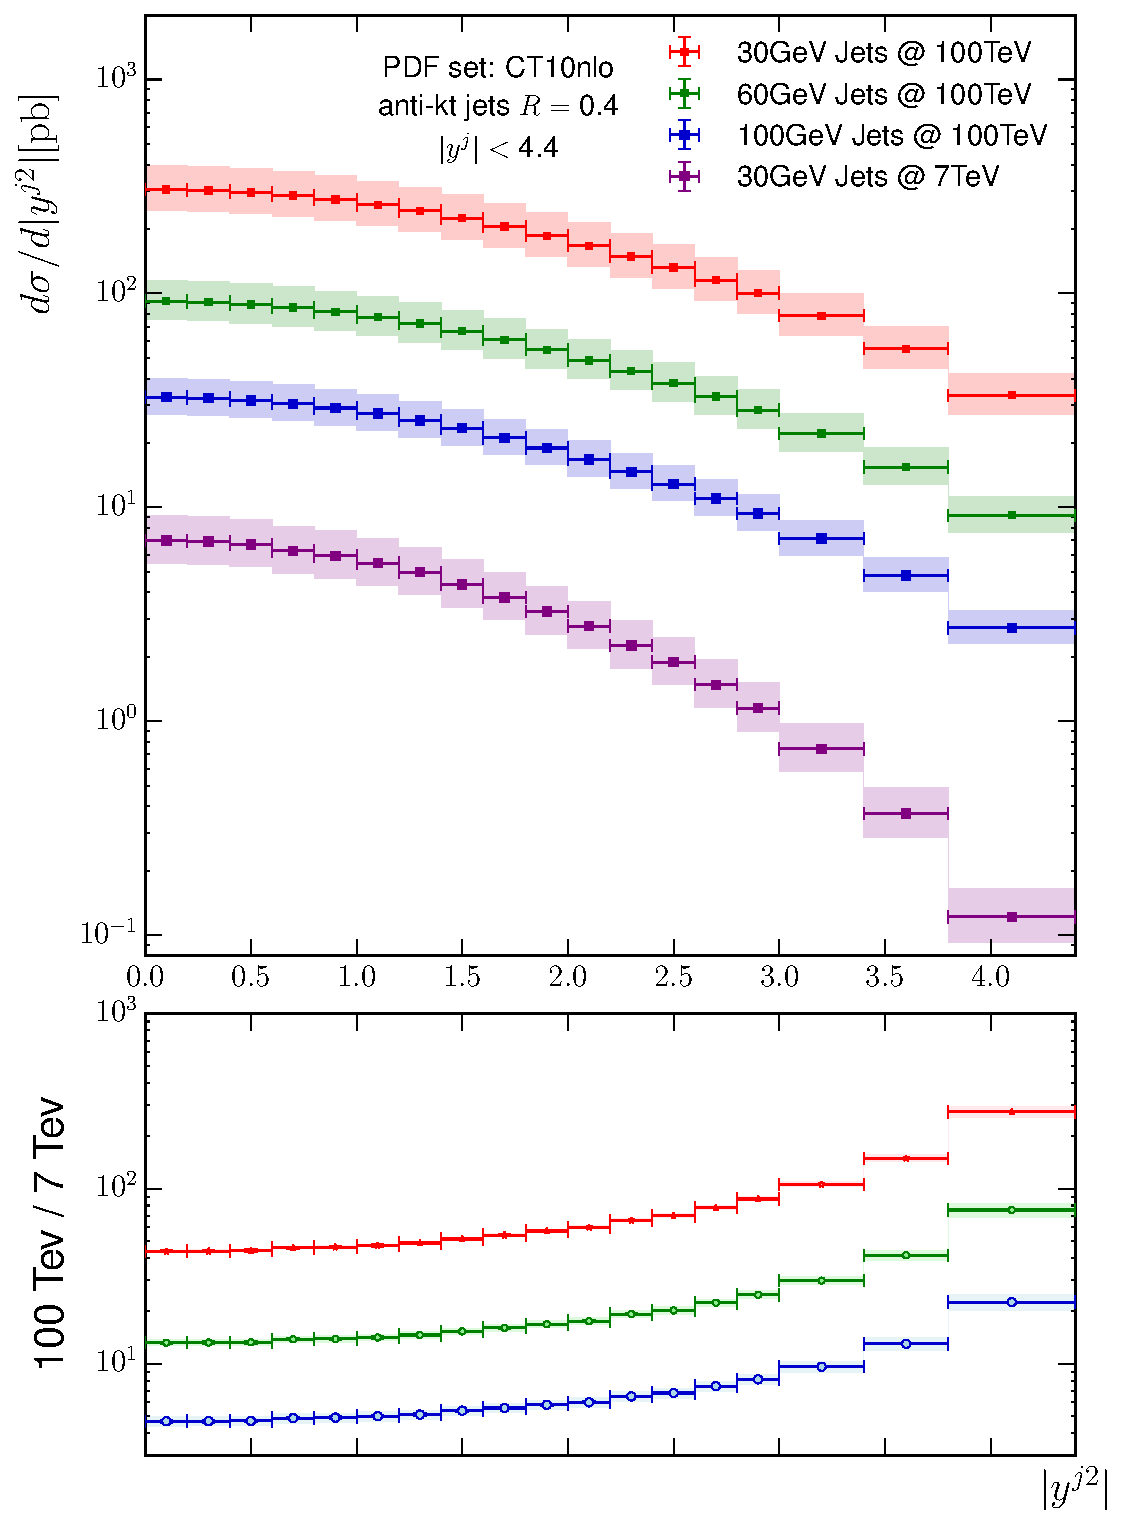
\includegraphics[width=\textwidth]{ATLAS_Z_100TeV_9b}
			\caption{}
			\label{fig:100tev_9b}
		\end{subfigure}

		\begin{subfigure}[b]{0.48\textwidth}
			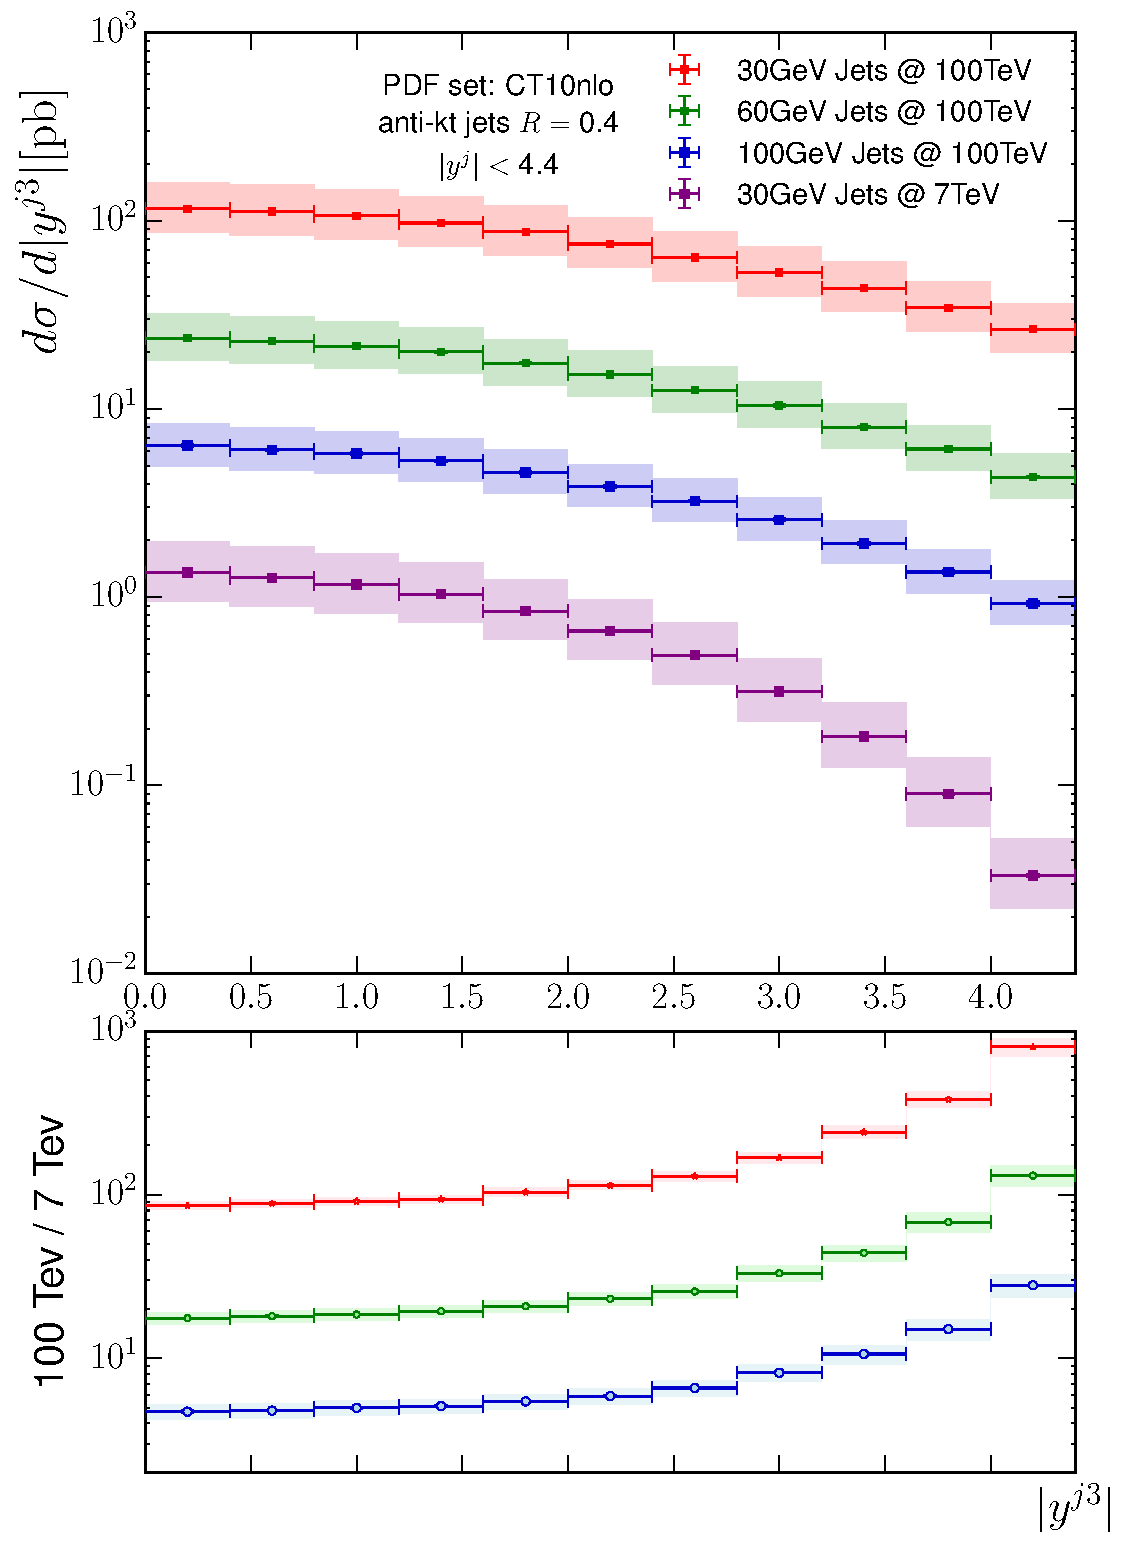
\includegraphics[width=\textwidth]{ATLAS_Z_100TeV_10a}
			\caption{}
			\label{fig:100tev_10a}
		\end{subfigure}
		~
		\begin{subfigure}[b]{0.48\textwidth}
			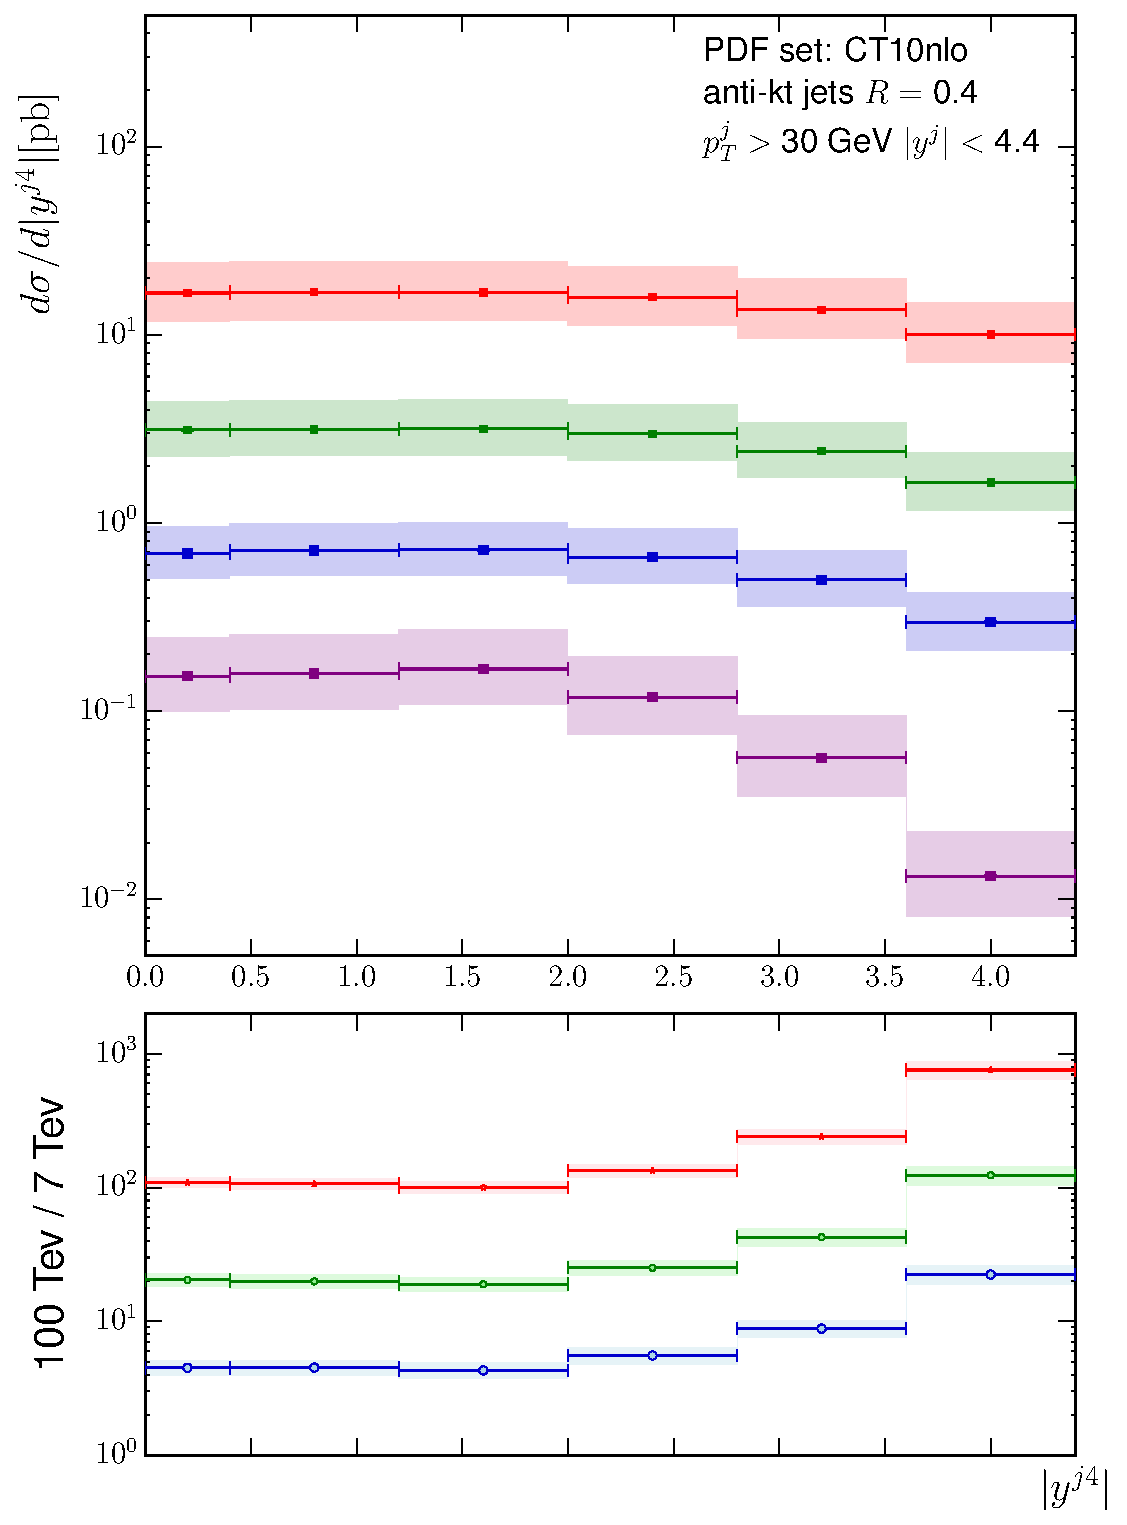
\includegraphics[width=\textwidth]{ATLAS_Z_100TeV_10b}
			\caption{}
			\label{fig:100tev_10b}
		\end{subfigure}
		\caption{The differential cross-section for $\zg$ plus inclusive dijets as a function of the absolute value of the rapidity
		         of the first, second and third leading jets in rapidity shown in fig. \eqref{fig:100tev_9b}, \eqref{fig:100tev_10a}
		         and \eqref{fig:100tev_10b} respectively and for centre-of-mass energies of 7TeV (blue) and 100TeV (pink).}
	\end{figure}

	Figs.~\eqref{fig:100tev_9b},~\eqref{fig:100tev_10a} and~\eqref{fig:100tev_10b} show the distributions in terms of
	the absolute value of the rapidity of the second, third and fourth leading jet in $p_\perp$.  Once again we observe
	the expected behaviour with an increase in QCD radiation at large values for rapidity at \htev relative to at \stev
	clearly visible.  In fig.~\eqref{fig:100tev_9b} we see that an increase in the jet $p_\perp$ cut has little effect
	on the shape of the ratio lines since there is still ample energy to access those rarefied regions of very forward
	and backward phase-space.  By contrast for figs.~\eqref{fig:100tev_10a} and~\eqref{fig:100tev_10b} we see that the
	higher jet cuts begin to take a toll on the jet activity at high values of $|y^j|$ and we see that the relative
	rates are suppressed in these regions.

	In summary, we see that the theoretical ideas discussed in chapters~\ref{chap:HEQCD},~\ref{chap:Zs} and~\ref{chap:ATLAS}
	and shown to be present in 7 and 8~TeV LHC data would be even more pervasive at a prospective high energy hadronic
	future circular collider.  The regions of phase space which are adequately described by fixed-order schemes at
	the (relatively) moderate energy ranges of the LHC would be impossible to describe correctly upon raising the energy
	to \htev.  We see that it is possible to somewhat protect the convergence of the QCD perturbative expansion by enforcing
	stringent jet transverse momentum cuts and that doing so would still lead to a significant increase in the measured
	total cross-section in $\zg$ plus dijet events.  However, even minimum jet $p_\perp$ cuts of 100~GeV are not sufficient
	to completely negate the effect of the large logarithmic corrections described in previous chapters.

